Los procesos de intercambio de opinión, donde las interacciones interpersonales influyen en la toma de decisiones, tienen amplia aplicación en estudios de comportamiento de las personas como por ejemplo en las ciencias sociales, políticas y económicas. Dichos procesos, son de gran interés para el estudio de procesos electorales en los cuales la opinión pública tiene directa injerencia en la decisión del electorado.

En este trabajo, continuaremos el estudio del impacto de los indecisos y su interacción con otros actores de opinión más fuerte y su consecuente impacto en el resultado de una elección bi-partidista. Extenderemos este trabajo enriqueciendo el comportamiento de los agentes, a través de modelar su capacidad de reaccionar ante eventos externos, que se disparan independientemente del estado de la dinámica de intercambio de opinión entre los agentes a los cuál estos afectan. A estos eventos los llamaremos \textbf{shocks de opinión}, que pueden pensarse como eventos que afectan un conjunto de agentes e influyen su opinión de manera exógena.

Entonces, a partir de la realización de esta extensión al modelo original, pretendemos ser capaces de modelar y analizar nuevos aspectos de la realidad, como por ejemplo el impacto de la influencia de los medios de información y las redes sociales en los indecisos del electorado promedio.

El objeto de estudio definido por Pina et.al es de una elección entre dos partidos (por ejemplo, en el ámbito de un ballotage presidencial), sometida a un libre intercambio de opiniones.

Los estados posibles de un agente, se encuentran en un intervalo de valores definido en el [-3, 3]. Donde los valores de [-3, -1) pertenecen a afinidad por el partido A, los valores entre [-1, 1] denotan que el agente se encuentra en estado de indefinición mientras que los valores en el intervalo (1, 3] son del partido B.
El motivo de esto es que el grado de convicción de los sujetos se encuentra en un espectro que puede variar a través del tiempo, debido a la dinámica de intercambio de opinión que se desarrolla en la población de células.

La grilla bidimensional de los agentes será de dimensión NxN. Para definir la interacción de cada individuo, se presenta una segunda capa en la grilla la cual contiene información sobre la conectividad de cada persona (ver \ref{fig:modelo_pina}). Cada sujeto modificará su estado en base a la información de la convicción de uno de sus primeros vecinos en las direcciones izquierda, derecha, arriba o abajo. Esto se define en una segunda capa de conectividad que cada determinado intervalo de tiempo genera un valor aleatorio en el rango [1, 4] que define de quien toma la influencia. A intervalos de tiempo de longitud Tau, toda la población recomputa su convicción.

\begin{figure}[!h]
\centering
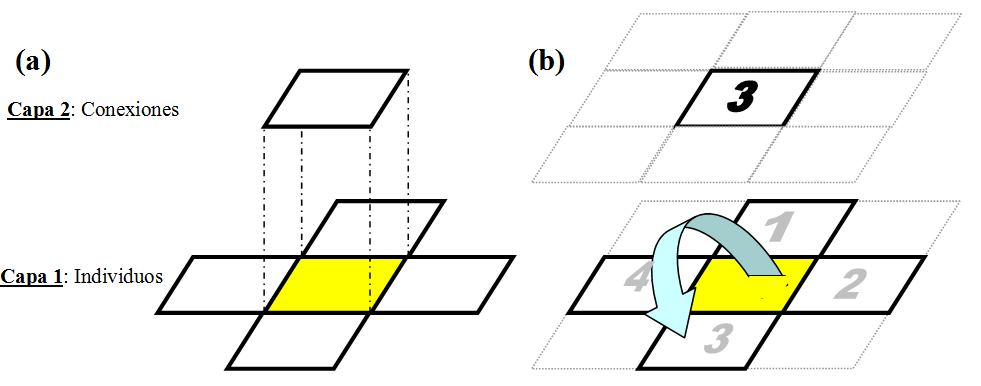
\includegraphics[scale=0.5]{imagenes/modelo_pina.png}
\caption{Vecindario de celdas utilizado para definir el comportamiento de cada agente}
\label{fig:modelo_pina}
\end{figure}

Para extender este vecindario, mediante los shock de influencia, definimos modelos atómicos DEVS que denominamos \textbf{shockers}. Estos interactúan con una cantidad fija de agentes de la grilla. En la figura \ref{fig:modelo_shockers} observamos 3 agentes shockers interactuando con 12 celdas cada una. Esta idea de que los atómicos interactúan con un subconjunto de la población de celdas nos permite generar esta influencia de manera dinámica y al tener varios shockers mejoramos la performance de ejecución al limitar la cantidad de puertos de salida que estos tienen. Además lo que observamos con esta decisión de diseño es que es posible variar el tipo de influencia que genera en torno a los grupos con los que interactúa. Por ejemplo con qué periodicidad inyecta un shock, o si el shock promueve la indecisión ó el extremismo hacia alguno o ambos partidos.

El comportamiento de los shockers está definido de la siguiente manera.

\begin{itemize}
\item Estos atómicos no mantienen un estado.
\item Los puertos de salida están conectados con un subconjunto de las celdas y esta interconexión no varía a lo largo del tiempo. Esta primer interconexión es elegida con distribución equiprobable.
\item En cada instante de tiempo en el cual se produce un shock, para cada shocker se selecciona con probabilidad uniforme un subconjunto de puertos de salida (dentro de sus celdas dominadas) y a estas se les envía una señal.
\item La periodicidad con la cual se realiza un shock forma parte de los parámetros del modelo y está definida en relación con el Tau definido para la interacción de los agentes.
\end{itemize}

\begin{figure}[!h]
\centering
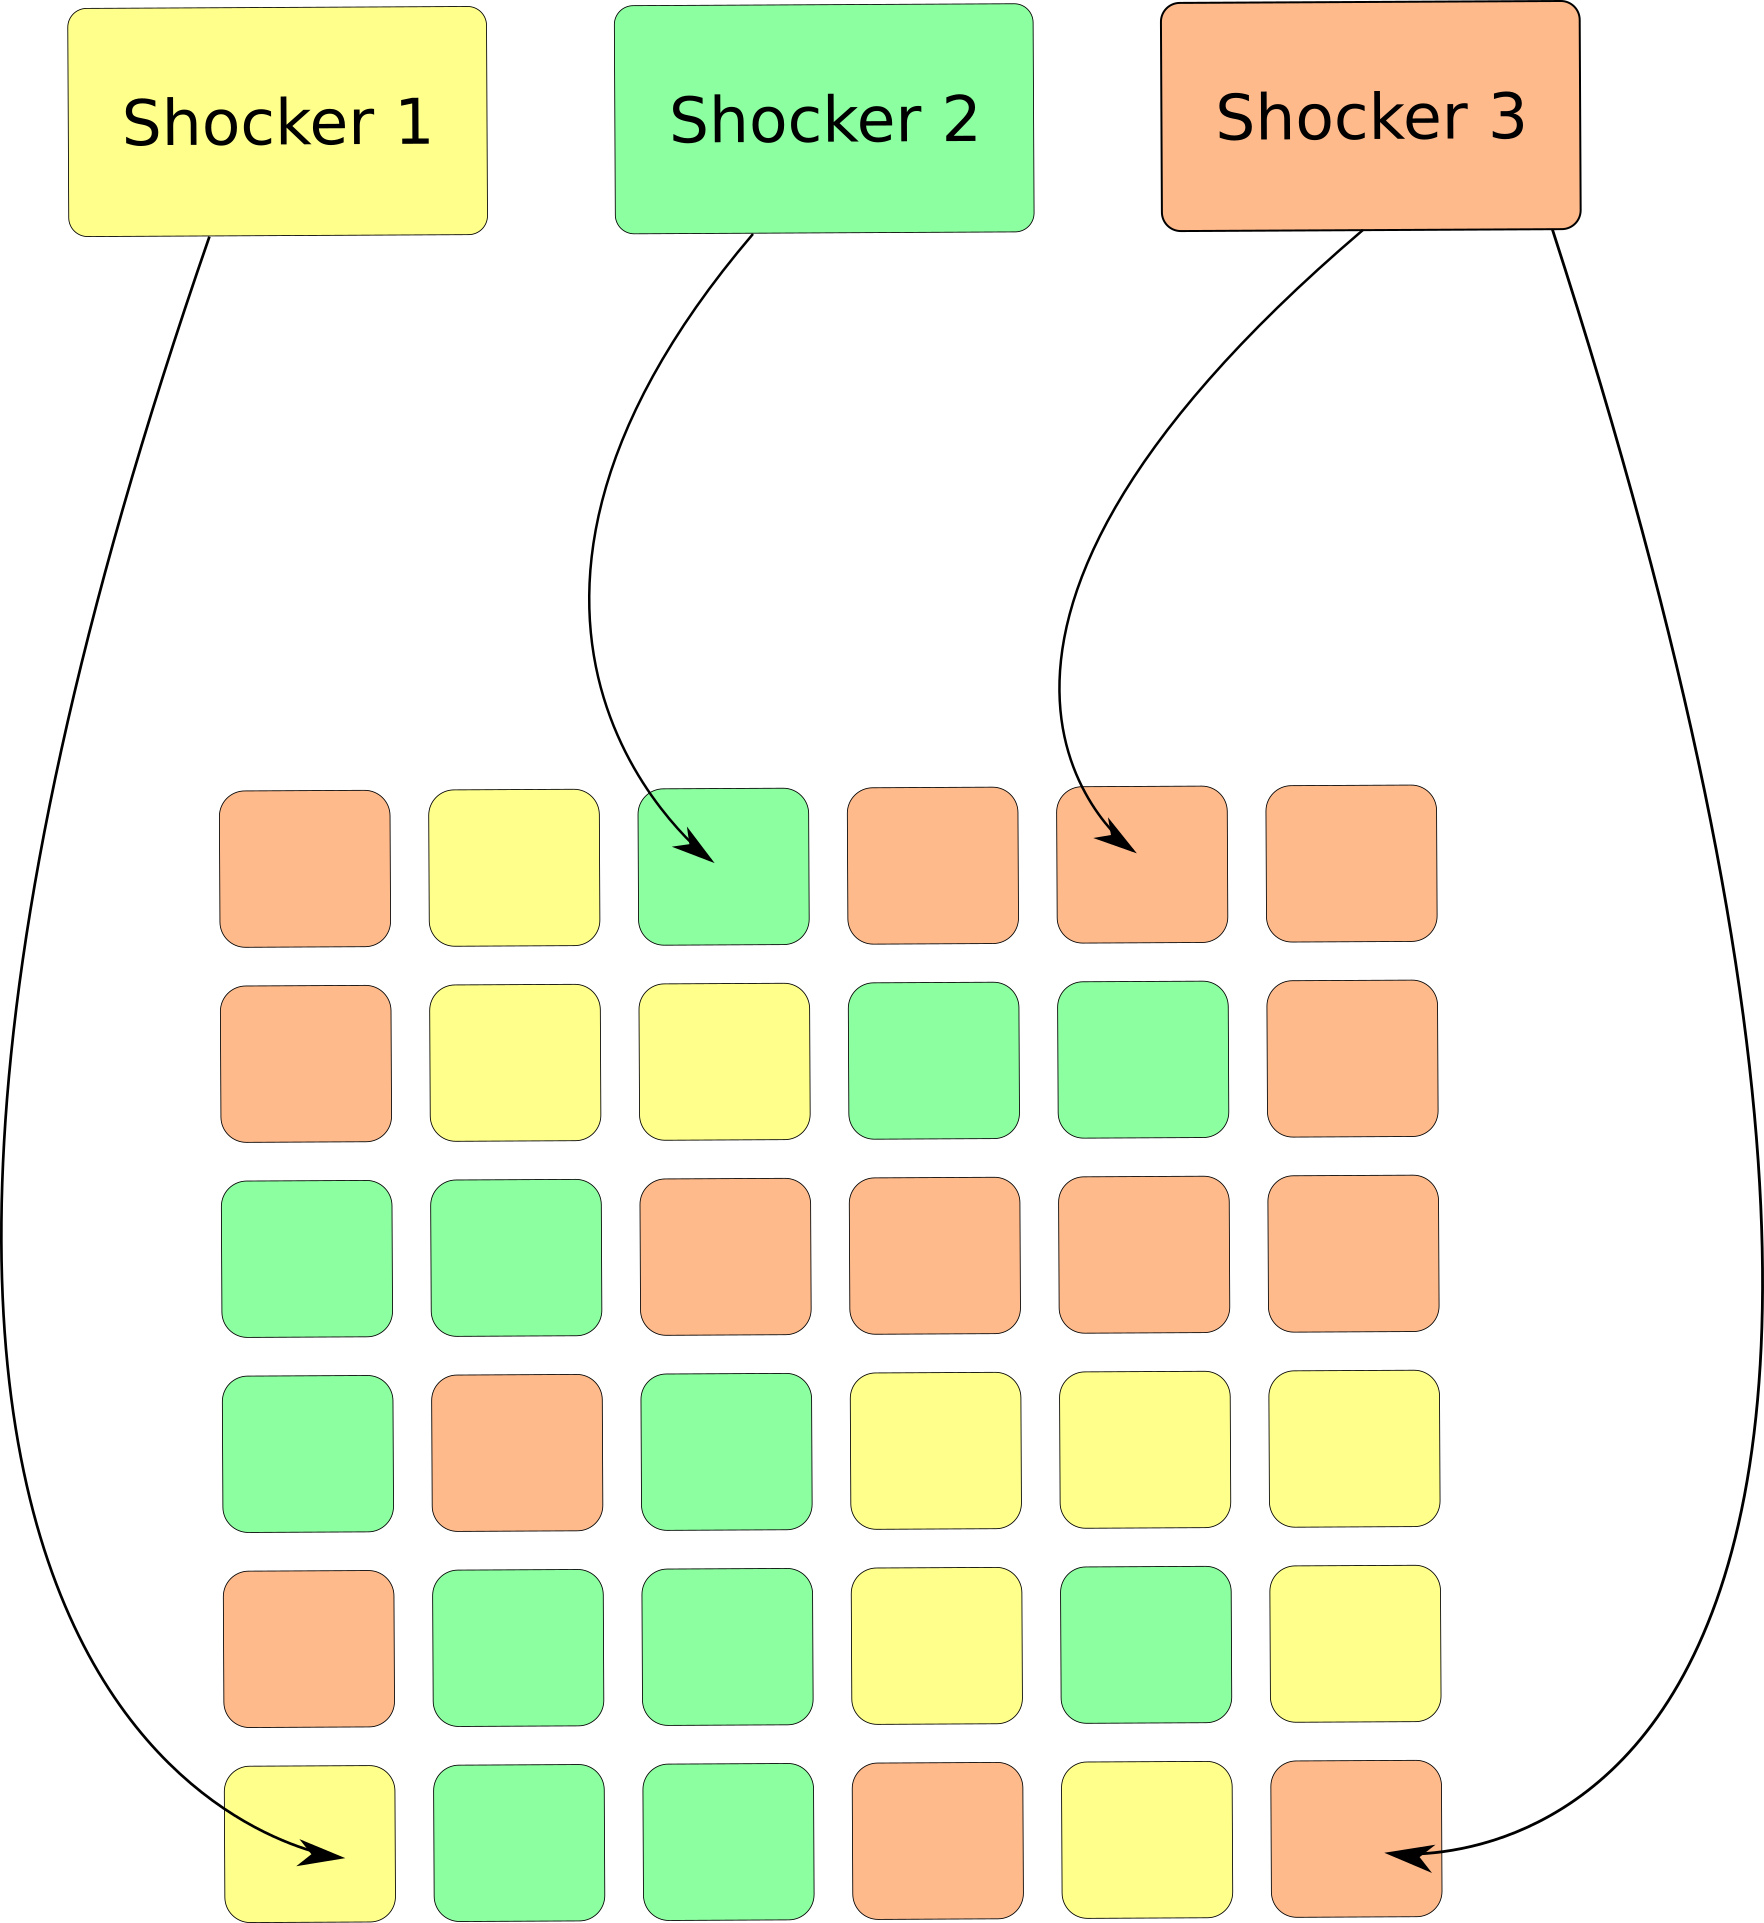
\includegraphics[scale=0.5]{imagenes/agentes_celdas_modelo.png}
\caption{Esquema que muestra el impacto de los shockers sobre el espacio celular}
\label{fig:modelo_shockers}
\end{figure}

Para los agentes, modificaremos su comportamiento. Al recibir una señal por el puerto de entrada, este definirá de manera aleatoria cómo se modifica su opinión. Su opinión variará en un delta, un coeficiente de corrimiento múltiplo del que los agentes utilizan al modificar su opinión durante sus interacciones con otros agentes.



